% =========================================================================
% ICRA 2027 submission: VSA cognitive maps (single-track paper)
% =========================================================================
% Class note: written against IEEEtran in conference mode, which Overleaf
% bundles. ICRA's PaperPlaza template is ieeeconf.cls (RAS template); the
% two are visually near-identical and switching is a one-line change:
%   \documentclass[letterpaper, 10pt, conference]{ieeeconf}
% plus dropping the IEEEtran-only options. Do the swap when the ieeeconf
% style files are added to the Overleaf project.
%
% MERGE NOTE (Paul): Sections I (Introduction) and VIII (Conclusion) are
% complete drafts written blind to the partial drafts already in this
% Overleaf project. Merge or replace, don't keep both.
%
% Every number in this file traces to the tracker
% (wiki/analysis/2026-07-29-vsa-query-layer-paper-plan.md) or a named
% artifact file. Provenance lives ONLY in "% provenance:" comments, so the
% rendered PDF shows real citations and URLs and never repo-internal
% pointers: the document is shared. Pending numbers are marked \todo{}.
% =========================================================================
\documentclass[conference]{IEEEtran}
\IEEEoverridecommandlockouts

\usepackage{amsmath,amssymb}
\usepackage{booktabs}
\usepackage{graphicx}
\usepackage{xcolor}
\usepackage{url}
\usepackage{cite}
% clickable references/URLs for the shared draft; drop if the PaperPlaza
% compliance check objects at submission time
\usepackage[hidelinks]{hyperref}
% cuted/capt-of removed 2026-08-18: the strip guaranteed page-1 hero
% placement but is fragile with two-column floats; a plain figure* on
% page 2 is the accepted trade.

% --- editorial TODO marker: strip before submission -----------------------
\newcommand{\todo}[1]{\textcolor{red}{\textbf{[TODO: #1]}}}
% binding / unbinding notation
\newcommand{\bnd}{\odot}
\newcommand{\conj}[1]{\overline{#1}}

\begin{document}

\title{Algebraic Spatio-Temporal Memory: a Fixed-Size Vector-Symbolic Map
with Exact Merge and a Predictive Capacity Law}

% Author order per Paul, 2026-08-10 ("Sven, Shay, Naitri, Lorin, then me,
% at least for now"). Surnames and affiliations verified from publication
% records except where marked \todo{}.
\author{
\IEEEauthorblockN{
Sven Krausse\IEEEauthorrefmark{1},
Shay Snyder\IEEEauthorrefmark{2},
Naitri Rajyaguru\IEEEauthorrefmark{3},
Lorin Achey\IEEEauthorrefmark{4},
Paul Kirkland\IEEEauthorrefmark{5}}
\IEEEauthorblockA{
\IEEEauthorrefmark{1}Peter Gr{\"u}nberg Institute, Forschungszentrum
J{\"u}lich, and RWTH Aachen University, Germany\\
\IEEEauthorrefmark{2}Parsa Research Laboratory, George Mason University,
Fairfax, VA, USA\\
\IEEEauthorrefmark{3}Perception and Robotics Group, University of
Maryland, College Park, MD, USA\\
\IEEEauthorrefmark{4}Collaborative AI and Robotics Lab, University of
Colorado Boulder, CO, USA\\
\IEEEauthorrefmark{5}International Centre for Neuromorphic Systems
(ICNS), The MARCS Institute, Western Sydney University, Australia\\
\todo{contact email for the corresponding author}}}

\maketitle


% =========================================================================
\begin{abstract}
Semantic maps on robots are usually structures that grow: a node per
object, a row per landmark, a descriptor per keyframe. We characterise
the opposite design point, a spatial-semantic map whose entire state is
one fixed-size vector. Observations are bound to positions by elementwise
complex multiplication over Fourier Holographic Reduced Representation
(FHRR) phasors, with continuous space encoded so that spatial
composition is an exact group operation, and superposed into a single
32\,KB trace ($D=8192$ unit-modulus phasors stored as phase angles alone,
one float32 per dimension; 64\,KB under the complex64 convention);
queries about objects, places and times are answered by the
algebra's inverse operation in milliseconds on a laptop CPU, with no
structure to traverse. Four properties are measured. Cross-traverse
relocalisation on 7-Scenes \texttt{chess} reaches 0.36\,m median 3D error
from the 32\,KB trace, against 0.29\,m for exact nearest neighbour over
the same descriptors at 32.8\,MB, in a size regime product quantisation
cannot enter. Object grounding across all eight Replica scenes leaves
zero memory-attributable misses against an explicit-instance ceiling.
Compactness is not the claim --- explicit representations now reach
kilobytes too --- the claim is that the size is fixed before deployment
and that degradation is predicted rather than silent.
Merging maps is vector addition: exact to floating-point reordering
($\sim$10$^{-15}$) and order-independent, where the equivalent
instance-association merge over identical observations needs 622 greedy
decisions and loses accuracy (84\% against 89\% mean grounding). And a
capacity law predicts a held-out condition to 1.4\%, having predicted a
deployed failure together with its fix (grounding 44\%$\to$62\%). The
memory does not exceed the ceiling its perception sets, and exact
merging assumes a shared coordinate frame.
\end{abstract}

% -------------------------------------------------------------------------
% PAGE-1 TEASER, as a "strip" rather than a figure*.
%
% Hero as a plain figure*: lands at the top of page 2 (LaTeX defers
% double-column floats past the page they are declared on); the page-1
% guarantee cuted provided was judged not worth its fragility
% (Paul, 2026-08-18).
% Regenerate with:  python tools/make_hero_figure.py
% Every photo, path, field and number is read from the measured inspector
% payloads; nothing is drawn by hand.
% -------------------------------------------------------------------------
\begin{figure*}[t]
\centering
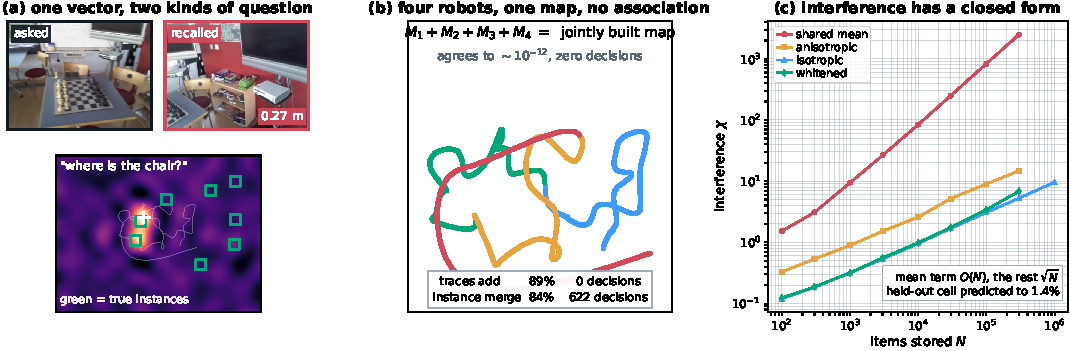
\includegraphics[width=\textwidth]{figures/hero.pdf}
\caption{\textbf{What the map \emph{is}.} Where a scene graph
accumulates a node per object and an edge per relation, this map is one
vector, and storing, querying and merging are arithmetic on it. Every
vector below is drawn as its phase angles, and every one was computed by
our implementation from the real Replica \texttt{room0} observation
stream.
\textbf{(a)} An observation is one multiply-add: a content atom is bound
to a fractional-power position code by an elementwise complex multiply
(Eq.~\eqref{eq:fpe}), and the product is added into a running sum.
\textbf{(b)} The whole map is that sum. All 8{,}028 detections of the
walk superpose into 8{,}192 phases at 4 bytes each, 32\,KB
(Sec.~\ref{sec:traces} on the byte convention), a size fixed before the
robot moves and unchanged by how much it then sees.
\textbf{(c)} A question is one unbind. Dividing by the \texttt{chair}
atom leaves a spatial belief \emph{field} over the floor rather than a
lookup result; the peak sits on a true instance, and the green squares
mark every ground-truth chair, including the ones a single argmax does
not resolve (Sec.~\ref{sec:limitations}).
\textbf{(d)} Four robots' maps combine by addition. The sum equals the
jointly built map to $10^{-11}$ with no data association whatsoever;
pooled over the eight Replica scenes it grounds 89\% against 84\% for the
equivalent explicit instance merge, which needs 622 greedy association
decisions to get there (Sec.~\ref{sec:merge-results}).}
\label{fig:hero}
\end{figure*}

% =========================================================================
\section{Introduction}
\label{sec:intro}
% MERGE NOTE: complete draft; merge with the Overleaf partial.

A mobile robot's semantic map is usually a data structure that grows: a 3D
scene graph adds a node per object and edges per relation
\cite{hughes2022hydra,gu2024conceptgraphs}, a landmark map adds a row per
landmark, a view database adds a descriptor per keyframe. Growth is not
the problem by itself; the machinery it obligates is. Updating a growing
structure means data association; merging two of them, across sessions
or across robots, means correspondence solving, outlier rejection, and
joint optimisation \cite{tian2022kimeramulti,chang2023hydramulti}; and
every downstream query needs code that \emph{traverses} the structure,
that is, walks it element by element (follow this object node, then its
edges, then test each neighbour) until it finds what the query asked
for, and that walking code is specific to the structure it walks.

Bounding that growth is now a named problem with its own survey. Across
roughly 52 systems from 1989 to 2025, Pangaliman et al.\
\cite{pangaliman2026memorysurvey} taxonomise spatial memory as dense,
sparse, neural or hierarchical-semantic, and quantify the gap between
stored map and runtime cost as the ratio of peak runtime memory to saved
map size --- a ratio reaching 215 for a 47\,MB neural map. Their critique of the systems that \emph{do} bound size is
the objection this paper must answer: hash-based maps cap the table, but
quality ``degrades silently when scene complexity approaches table
capacity, providing bounded memory rather than constant-quality
scaling.'' Fixed size is therefore not the contribution on its own.
\emph{Predicted} degradation is: the capacity law of Sec.~\ref{sec:law}
says when the trace saturates, by how much, and what to do about it, and
it called one such failure in advance of our finding it.

This paper characterises the opposite design point: a map that does not
grow. A robot that has driven for an hour and a robot that has driven for
a week hand over the same object, 8{,}192 phase angles at four bytes
each, and the cost of querying it has not moved either. We build that
object from a vector symbolic algebra (VSA; the older literature reads
the acronym as ``architecture''), used as an \emph{algebraic composition
layer}. Class, appearance, position, heading and time are each encoded as
high-dimensional unitary phasor vectors, composed by one binding
operator, and superposed into a map state whose size is fixed
\emph{before} the robot ever moves: 32\,KB in every experiment here. The
naming distinction is worth keeping: the algebra supplies the operators
(bind, bundle, unbind), and the map is the architecture we build from
them. Insertion is one multiply-add, $O(D)$. A family of
spatial-semantic queries (``where was a chair?'', ``what is at
$(x,y)$?'', ``when was this place occupied?'') is answered by the
algebra's inverse operation, a single unbind followed by a kernel
readout; nothing ever walks a structure, because there is no structure to
walk. Merging two maps is elementwise addition of two vectors:
commutative, associative and exact, because a representation that makes
no association decisions has none for a merge step to get wrong.

Properties that are usually separate subsystems therefore arrive as
identities of the algebra, and we measure each one on real data
(Fig.~\ref{fig:hero}). \emph{Query} is one unbind, milliseconds on a
laptop CPU.
\emph{Relocalisation} from the 32\,KB trace reaches 0.36\,m median error
on the official 7-Scenes \texttt{chess} cross-traverse split, against
0.29\,m for exact nearest neighbour over the same descriptors at
32.8\,MB, and product quantisation cannot occupy that size regime at all
because its codebook alone is $\sim$2\,MB. \emph{Merge} is addition, and
it is exact in a checkable sense: four session memories built
independently from separate traverses, summed, answer all 2{,}000 test
queries identically to the jointly built map. \emph{Filtering} is one
bind and one bundle, which caps drift where dead reckoning diverges. And
because everything shares one superposition, the memory's interference
has a closed form: a capacity law that predicts a held-out condition to
1.4\% and that predicted a class-imbalance failure on real scenes
together with the bounded-insertion fix that repaired it.

We are equally explicit about what is not claimed. The memory does not
out-localise a nearest-neighbour search over its own input descriptors;
superposition is lossy, and lossy representations lose. A detector-fed
object memory cannot label the walls and floors that dominate dense
semantic-segmentation benchmarks, so we pre-register that expectation
under the target benchmark's own scorer rather than choosing a protocol
that hides it (Sec.~\ref{sec:grounding}). Exact merging assumes a shared
coordinate frame, which is precisely what the classical merge machinery
exists to recover; the algebra assumes the frame, it does not solve it.
Instance identity is a stated limitation. The claims are about what a
fixed-size algebraic map state buys \emph{at the ceiling its perception
sets}: recall within 0.07\,m of exact nearest neighbour at
$\sim$1000$\times$ fewer bytes, grounding across eight scenes whose
misses are entirely perceptual, drift bounded by a filter that runs
wholly in the algebra, and a merge operator whose cost and exactness no
growing representation matches.

Contributions:
\begin{enumerate}
\item \textbf{System} (Sec.~\ref{sec:method}): a fixed-dimensional
  associative map over real perception: FHRR traces with fractional
  power encoding, a multi-trace layout matched to query families, bounded
  per-class insertion, and a content-conditioning discipline (centre or
  z-score, or bind a diverse key; the two are measured substitutes).
\item \textbf{Capacity law} (Sec.~\ref{sec:law}): an empirical law for
  superposition interference, $\chi(N)$, separating a mean term, a
  quadrature content/projection term, and a temporal-persistence factor;
  it predicts a held-out condition to 1.4\%, diagnosed a deployed
  failure, and predicted the direction of its fix.
\item \textbf{Benchmark characterisation} (Sec.~\ref{sec:results}):
  cross-traverse relocalisation on 7-Scenes \texttt{chess} against
  storage-matched and storage-unmatched baselines; object grounding on
  all eight Replica scenes with a full miss taxonomy; a head-to-head
  against ConceptGraphs under its own evaluation, baseline reproduced
  to 99\% of published first, in which the bounded memory overtakes the
  unbounded map in every degraded-input condition tested; drift bounding
  under a 20$\times$ odometry-degradation sweep.
\item \textbf{Exact merge} (Sec.~\ref{sec:merge-results}): map merging as
  vector addition, measured against an instance-association merge, count
  grids, and raw-data union on identical observations. Bundling as a
  between-robot merge operator was demonstrated for occupancy by VSA-OGM
  \cite{snyder2026vsaogm}; we carry it to a bound spatial-semantic memory
  and supply what a fused-accuracy number cannot: a measured agreement
  check against the jointly built map, a head-to-head against
  association-based merging on identical observations, and a count of the
  association decisions avoided --- with the shared-frame assumption it
  rests on stated plainly.
\end{enumerate}

% =========================================================================
\section{Related Work}
\label{sec:related}

\textbf{Vector symbolic algebras.} Holographic reduced
representations \cite{plate1995holographic} and hyperdimensional
computing \cite{kanerva2009hyperdimensional,kleyko2022survey} compose
symbols in a fixed-dimensional space via binding and superposition
(the surveys use the older reading ``vector symbolic architectures''),
with capacity analyses assuming i.i.d.\ quasi-orthogonal vectors
\cite{frady2018theory}. Continuous space enters through fractional power
encoding (FPE) / spatial semantic pointers
\cite{komer2019neural,voelker2021simulating}, deployed in spiking form by
SSP-SLAM \cite{dumont2023sspslam}, and as a grid-cell-inspired structured
vector algebra by Krausse et al.\ \cite{krausse2025gcvsa} (synthetic
data). Our contribution to this
lineage is deployment-side: real perception features violate the
randomness assumptions (Sec.~\ref{sec:law}), and we provide the
conditioning rules and the capacity law that make the algebra work on
them. HDC aggregation of image descriptors exists \emph{within} an agent
for place recognition \cite{neubert2021hyperdimensional} and across
clients in federated learning \cite{fedhd2022}. Closest to us, VSA-OGM
\cite{snyder2026vsaogm} already merges maps \emph{between} robots by
bundling, on a synthetic LiDAR scene (2 agents) and Intel Campus
quadrants (4 agents), reporting fused AUC 0.95 at roughly one point
cloud's processing cost. Two differences set our result apart. What is
merged: VSA-OGM bundles occupancy --- binary occupied/empty classes over
a tiled grid of memory vectors --- where we bundle a spatial-semantic
memory binding class, appearance, position, heading and time. And what is
measured: VSA-OGM reports fused accuracy, not exactness, and does not
compare against an association-based merge over identical observations
(Sec.~\ref{sec:merge-results}). VSA-OGM also \emph{tiles} rather than
bundling into one vector, because a single trace weights all regions
equally, and lists memory-vector saturation as an open limitation; the
capacity law of Sec.~\ref{sec:law} is what lets us keep the single
fixed-size trace and say in advance when it will fail.

\textbf{Scene graphs and open-vocabulary maps.} Hydra
\cite{hughes2022hydra}, ConceptGraphs \cite{gu2024conceptgraphs},
ConceptFusion \cite{jatavallabhula2023conceptfusion}, HOV-SG
\cite{werby2024hovsg} and successors \cite{keysg2025} build exact,
mutable, relational structures with open-vocabulary semantics; planners
operate on them directly \cite{agia2022taskography}. These systems and
ours occupy different corners of a real trade-off: exact/mutable/growing
state versus bounded/associative/approximate state. Two 2026 results
sharpen that trade-off in the graphs' favour on bytes, and we state it
rather than let a reviewer state it for us. Clio \cite{maggio2024clio}
compresses a graph by an agglomerative information bottleneck over
natural-language tasks, keeping only task-relevant granularity;
LOST-3DSG \cite{ferraina2026lost3dsg} replaces dense CLIP attributes
with word2vec and sentence embeddings, representing a 21-object scene in
3{,}297 bytes --- an order of magnitude below our trace, with instance
identity intact, which is exactly what Sec.~\ref{sec:limitations}
concedes we lack. Small is therefore no longer the differentiator, and
we do not argue it: what no explicit representation offers is a
footprint fixed \emph{before} deployment, an update cost independent of
map age, and a merge cost independent of map content. We adopt
ConceptGraphs' own evaluation for the semantic comparison
(Sec.~\ref{sec:grounding}) rather than inventing a metric. Relational
spatial memories with referring-expression interfaces \cite{farm2026}
mark the expressiveness frontier this representation does not yet reach
(Sec.~\ref{sec:limitations}).

\textbf{Relocalisation.} Retrieval-based relocalisation stores a
descriptor database and returns the pose of the best match
\cite{sattler2019understanding}; compression via product quantisation
\cite{jegou2011product} trades accuracy for bytes but is floored by its
codebook. We use 7-Scenes \cite{shotton2013scene} with EigenPlaces
descriptors \cite{berton2023eigenplaces} and treat exact nearest
neighbour over the same descriptors as the ceiling the memory should
track.

\textbf{Multi-robot map merging.} Every established family pays for
merging: occupancy grids need transform search then cell-wise fusion
\cite{birk2006merging,carpin2008fast}; pose-graph systems need
inter-robot loop closures, outlier rejection, and distributed
optimisation
\cite{cunningham2010ddfsam,mangelson2018pcm,lajoie2020doorslam,tian2022kimeramulti,cramariuc2023maplab,lajoie2024swarmslam},
moving 24--146\,MB per experiment in Kimera-Multi's reporting
\cite{tian2022kimeramulti}; scene graphs additionally need per-layer node
association \cite{chang2023hydramulti}; submap joining propagates dense
covariance \cite{tardos2002robust,huang2008slsjf,zhao2019linear}; neural
implicit maps need consensus optimisation over many communication rounds
\cite{hu2023cpslam,dinerf2024,magicslam2025}. All produce estimates:
order- and iteration-dependent, never bit-identical to a jointly built
map, with association errors that persist. Table~\ref{tab:merge-survey}
summarises. The VSA trace makes the merge step itself trivial and exact;
what it does \emph{not} solve, the shared reference frame the classical
machinery exists to recover, is stated as a standing caveat in
Sec.~\ref{sec:merge-results}.

\begin{table}[t]
\caption{Map merging across representation families; communication and
exactness refer to the merge step given established relative poses.
Representative systems for each family are cited in
Sec.~\ref{sec:related}.}
\label{tab:merge-survey}
\centering
\small
\begin{tabular}{@{}p{2.1cm}p{2.6cm}p{2.9cm}@{}}
\toprule
Family & Merge operation & Cost / exactness \\
\midrule
Occupancy grids & cell-wise fusion after SE(2) search & $O$(area$\times$res) comms; approximate \\
Pose/factor graphs & joint optimisation over stitched graph & 24--146\,MB per expt.\ \cite{tian2022kimeramulti}; estimate \\
3D scene graphs & per-layer node association + re-optimisation & association errors persist \cite{chang2023hydramulti} \\
Task-compressed graphs & association, then re-run compression & bottleneck is task-specific \cite{maggio2024clio} \\
Neural implicit & consensus optimisation & many rounds; may diverge \\
\textbf{VSA trace (ours)} & \textbf{elementwise addition} & \textbf{one 32\,KB vector; exact, commutative, associative} \\
\bottomrule
\end{tabular}
\end{table}

% =========================================================================
\section{Method: the Algebraic Map}
\label{sec:method}

\subsection{Encoding: FHRR phasors and fractional power encoding}
\label{sec:encoding}

All atoms are unitary phasor vectors $z \in \mathbb{C}^{D}$ with
$z_j = e^{i\theta_j}$, $\theta_j \sim \mathcal{U}[-\pi,\pi)$, at
$D=8192$ throughout. Binding is the elementwise (Hadamard) complex
product $a \bnd b$; unbinding is binding with the conjugate,
$a \bnd \conj{a} = \mathbf{1}$; superposition is vector addition. A
discrete symbol (a class name, an appearance prototype) is one random
atom; continuous quantities use \emph{fractional power encoding}
\cite{komer2019neural}: a base atom $X$ is exponentiated elementwise,
\begin{equation}
S(x) \;=\; X^{x} \;:=\; e^{\,i x \boldsymbol{\theta}_X}, \qquad
S(x,y) = X^{x} \bnd Y^{y},
\label{eq:fpe}
\end{equation}
which makes position encoding a group homomorphism:
\begin{equation}
S(a) \bnd S(b) \;=\; S(a+b).
\label{eq:homo}
\end{equation}
Property~\eqref{eq:homo} holds to machine precision in our implementation
(max elementwise deviation $1.5\times10^{-16}$ between an unbind-shifted
field and the physically re-encoded field, over a $4\times4$ displacement
sweep); translation of a whole belief field costs one bind. The
similarity $\langle S(x), S(x')\rangle$ is a fixed radial kernel whose
length-scale $\ell$ is set by the bandwidth of
$\boldsymbol{\theta}_X$; we use $\ell$ in the 0.5--0.75\,m range
indoors. Heading uses a circular base atom with integer frequencies
$\pm\{1,2,3\}$ and \emph{no DC component}, so that summing an encoded
heading over the full circle annihilates: marginalising heading out of a
query costs one bundled probe rather than a sweep.

\subsection{Map state: traces}
\label{sec:traces}

An observation at time $t$, a content vector $c$ (a class atom, an
appearance phasor, or their binding) at position $(x,y)$, is inserted
into a trace by one multiply-add:
\begin{equation}
M \;\leftarrow\; M + c \bnd S(x,y).
\label{eq:insert}
\end{equation}
A query for content $c$ produces a spatial belief field by unbinding and
kernel readout,
\begin{equation}
f(x) \;=\; \operatorname{Re}\,\langle\, M \bnd \conj{c},\; S(x)\,\rangle,
\label{eq:field}
\end{equation}
evaluated over a display grid; the answer is the field's argmax, and we
recommend reporting the top-$k$ modes (Sec.~\ref{sec:setup}). The field
\emph{is} the map; argmax is one readout of a full spatial belief.
This bind-then-bundle write and its inverting query are not new to us:
HyperSpace \cite{snyder2026hyperspace} formalises the same pair as the
storage and query modules of a general spatial-VSA framework
($m \leftarrow m \oplus (\phi_p(x) \otimes \phi_v(v))$, queried by
positional inversion, cleanup and regression). We take the primitive as
given and ask what a \emph{fixed} budget of it buys on real perception.

Because a trace answers best the query shape it was built for, the memory
keeps one trace per query family, in effect the algebra's secondary
indexes:
$M_{\text{what-where}} = \sum c \bnd S(x)$,
$M_{\text{what-when}} = \sum c \bnd T(t)$,
$M_{\text{where-when}} = \sum S(x) \bnd T(t)$, and the full event trace
$M_{\text{event}} = \sum c \bnd S(x) \bnd T(t)$ for two-factor-cued
queries. Writes fan out ($O(D)$ each); each trace carries its own
capacity budget under the law of Sec.~\ref{sec:law}. Temporal
\emph{range} queries use closed-form range kernels
$T_{[a,b]} = \int_a^b T^{t}\,dt$ (per-frequency closed form), so a time
interval costs the same one unbind as a time point. At $D=8192$, one
trace is 8{,}192 phase angles at 4 bytes: 32\,KB. \emph{Byte convention
(load-bearing).} Because the phasors are unit-modulus, the map state is
the phase angles alone, one float32 per dimension. The standard FHRR
accounting stores a complex64 pair per dimension and would give
$8D = 64$\,KB \cite{snyder2026hyperspace}; the magnitudes it stores are
the constant we never need. Every byte count in this paper uses the
phase-only convention, and doubling them recovers the complex64 reading.
Footprint honesty:
the trace is the \emph{map state}; the decode grid used to display a
field is working memory derived from the shared basis, and dense decoding
dominates query latency ($\sim$91\% in profiling) but is not needed by
consumers that stay in the algebra, such as the drift filter of
Sec.~\ref{sec:kalman-results}. HyperSpace
\cite{snyder2026hyperspace} measures the same effect independently and
from a different pipeline: similarity-driven cleanup and regression
dominate end-to-end runtime in spatial domains, to the point where HRR
and FHRR come out comparable despite FHRR's cheaper operators. The
saving is available only to consumers that never decode. Query latency is milliseconds on a laptop
CPU (2.7--15\,ms measured across our configurations at $D=4096$--8192).

\subsection{Bounded per-class insertion}
\label{sec:bounded}

Class frequencies in real streams are heavy-tailed, and the capacity law
predicts the consequence: a class stored 1{,}150 times buries one stored
5 times under crosstalk mass (Sec.~\ref{sec:law}). Insertion is therefore
capped per content symbol (reservoir-style, $\le 60$ insertions per
class), which is online, requires no second pass, and preserves merge
exactness by construction. On Replica \texttt{room0} this raised
provisional consistency-R@1 from 44\% to 62\% (all classes) exactly as
the law's direction predicted; the final truth-scored protocol grounds
5 of 6 GT-comparable classes (83\%).
% provenance: tracker (ba->bb); outputs/replica_room0/object_grounding.json
% (metric 'truth'); the 44->62 pair is the provisional consistency metric

\subsection{Content conditioning, and a substitution law}
\label{sec:conditioning}

Learned perception features violate the i.i.d.-random assumption of VSA
capacity theory in one dominant way: a shared mean direction that
accumulates \emph{coherently} across stored items
(Sec.~\ref{sec:law}). Two measured rescues exist, and they substitute for
each other:
\begin{enumerate}
\item \textbf{Condition the content stream}: centre, or z-score per
  dimension, using statistics fit on the memory-building data only
  (never the queries). Full whitening is \emph{not} a stronger version of
  this fix: it flattens the spectrum, which is where retrieval lives,
  and scores below a constant predictor in most of our held-out cells
  (e.g.\ $-47.6\%$ signal, classroom EigenPlaces, 5 seeds); its effect
  is scene- and encoder-dependent (it is harmless on \texttt{chess}), so
  we state it as scoped, not universal.
\item \textbf{Bind a diverse key}: adding a third bound factor whose
  value varies across insertions (e.g.\ heading) scatters the shared
  mean's phases, destroying the coherent pile-up \emph{by the key}
  rather than by preprocessing. On streams where content is nearly
  parallel this rescues a degenerate memory outright ($-38.7\%$
  signal, decode collapsed to one cell $\to$ $+63.3\%$; classroom
  YOLOv8n).
  % provenance: tracker (am)
\end{enumerate}
Use exactly one. Binding an \emph{uninformative} extra key when content
is already conditioned adds pure crosstalk (0.35\,m $\to$ 1.00\,m on
classroom EigenPlaces); whether a key is informative is
trajectory-dependent (heading helps on an orbit-style traverse,
Sec.~\ref{sec:chess}).

\subsection{Merge}
\label{sec:merge-method}

Two traces built under a shared atom vocabulary (same basis seeds) and a
shared coordinate convention merge by elementwise addition:
$M_{A\cup B} = M_A + M_B$. The operation is commutative, associative,
content-independent in cost (one $D$-vector per robot), and exact: it
is the same sum a jointly-built map would have computed, up to
floating-point reordering. There are no association decisions because
there are no discrete elements to associate. What addition does
\emph{not} provide is the shared frame itself: aligning coordinate
conventions is precisely the problem the classical merge machinery
solves, and misaligned traces sum to a superposition of inconsistent maps
with no error signal. All merge results in this paper assume the frame
(Sec.~\ref{sec:merge-results}); recovering it inside the algebra is
future work.

% =========================================================================
\section{A Predictive Capacity Law}
\label{sec:law}

\subsection{Metric}
Store $N$ items, probe with a stored key, and measure the response at
non-target locations in units of one item's on-target signal:
\begin{equation}
\chi(N) \;=\; N \cdot \operatorname{mean}_i \left| \text{off-target}_i \right|,
\label{eq:chi}
\end{equation}
the interference amplitude per unit item signal ($\chi$ values are
comparable only at matched $N$). Retrieval flips when interference mass
competes with the on-target peak, so $\chi$'s growth in $N$ \emph{is} the
capacity story. This is the quantity whose absence forces tiling
elsewhere: VSA-OGM \cite{snyder2026vsaogm} partitions the environment
into per-region memory vectors and records saturation --- dimensionality
or tile count having to grow with point count --- as an open limitation.
A law for $\chi$ is what lets a single fixed-size trace stay single.

\subsection{The law}
Across controlled synthetic sweeps ($N$ to $10^6$;
Fig.~\ref{fig:law}) and real encoder streams, interference follows
\begin{equation}
\chi(N) \;=\; a_\mu N \;+\; \sqrt{N}\,
\sqrt{\tfrac{\alpha}{\mathrm{PR}_{\mathrm{eff}}} + \tfrac{\gamma}{D}}\;
h(N,\tau),
\label{eq:law}
\end{equation}
with three separately-evidenced components:
% provenance: tracker (az); wiki/analysis/2026-08-04-t1-chi-law-empirics.md;
% outputs/synthetic/rows.jsonl + outputs/synthetic_hd1024/rows.jsonl
\begin{itemize}
\item \textbf{Mean term, exactly linear.} A shared mean direction adds in
  phase: $\chi/N$ is constant to $3\times10^{5}$ items (0.0083 across the
  sweep); configurations without a mean fit $a_\mu \approx 0$. This term
  never bends; it is the component the conditioning rules of
  Sec.~\ref{sec:conditioning} exist to kill (centring removes it,
  a diverse bound key phase-scatters it, which is the mechanism behind
  the substitution law).
\item \textbf{Quadrature fluctuation term.} The $\sqrt{N}$ prefactor has
  two sources in quadrature: content-space overlap $\alpha/\mathrm{PR}$
  (participation ratio of the content covariance; treatments act here)
  and a projection-noise floor $\gamma/D$ that is
  \emph{content-independent}. A single-power-law alternative was
  falsified by a $D$=1024 run; the quadrature model fits all
  (config$\times D$) cells and predicts a held-out cell to
  \textbf{1.4\%} (predicted 0.0321, observed 0.0316). The $\gamma/D$
  term explains a real-data observation: after whitening, four backbones
  spanning raw $\chi$ 79.8--201.8 (YOLOv8n, ResNet-50, DINOv2-S,
  untrained ResNet-50; $N$=2{,}429, $D$=8192) land on the same floor
  ($\chi$ 9.1--11.0): no content treatment can go below the
  projection floor; only more dimensions can.
\item \textbf{Persistence factor.} Temporally correlated streams grow
  coherently while $N \lesssim \tau$ (the correlation length in items),
  then revert to $\sqrt{N}$ with a \emph{permanent} elevation
  $h_\infty = \sqrt{1 + \tau/\tau_0}$ ($\tau_0 \approx 60$ at our
  settings; elevation$^2-1 \propto \tau$ verified across a 200$\times$
  range of $\tau$). The mean is the $\tau\to\infty$ limit. Practical
  consequence: naive $O(N)$ extrapolation from small-$N$ measurements
  \emph{overstates} crosstalk at scale for everything except the mean
  term.
\end{itemize}

\begin{figure}[t]
\centering
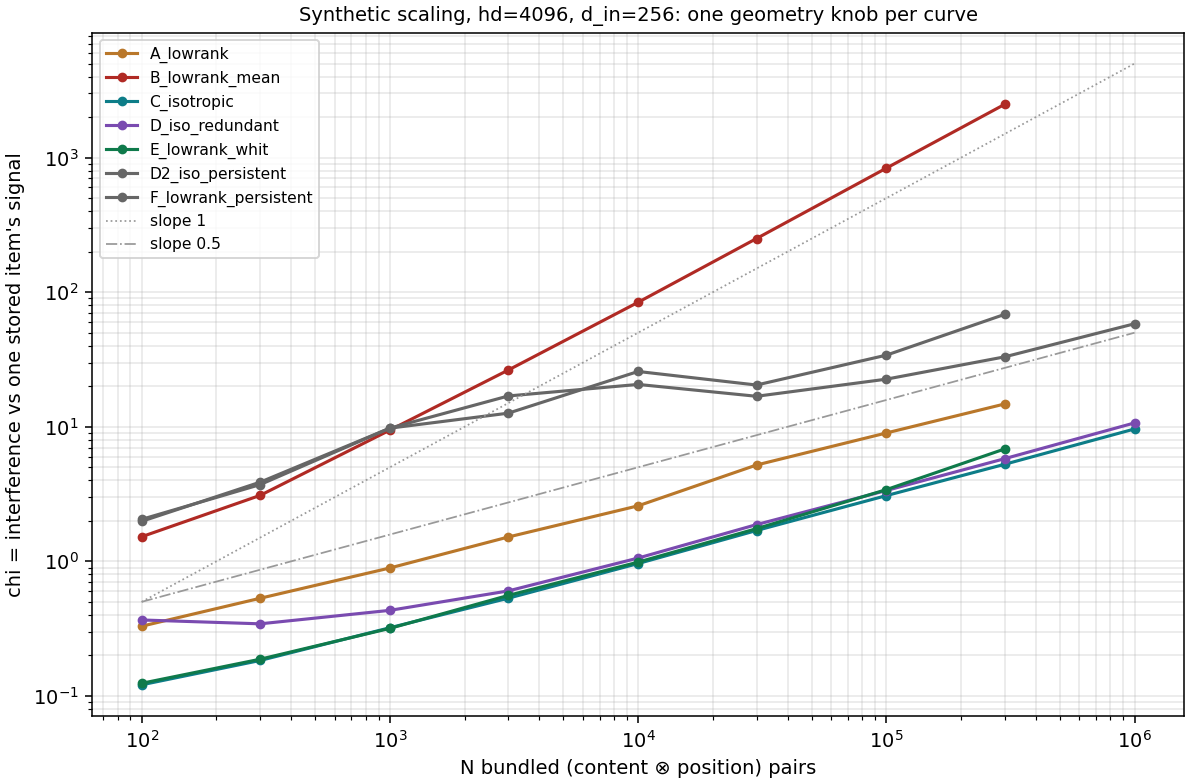
\includegraphics[width=\linewidth]{figures/synthetic_scaling.png}
\caption{Interference growth $\chi(N)$ on controlled synthetic content
streams through the exact deployed pipeline. A shared mean grows
coherently ($O(N)$, never bends); anisotropic-but-independent content
grows at $\sqrt{N}$ with a larger prefactor; temporally persistent
content is transiently coherent then reverts. These are the three terms
of Eq.~\eqref{eq:law}. \todo{regenerate with final styling + legend
labels matching the equation terms}}
\label{fig:law}
\end{figure}

\subsection{Deployed predictions}
The law is not descriptive bookkeeping; it called failures in advance.
(i) \emph{Class imbalance}: heavy-tailed insertion counts put a large
coherent mass on frequent classes (the trace-level mean term at class
granularity), predicting that rare classes drown. Measured: couch at
1{,}150 insertions buried book at 5; bounded insertion
(Sec.~\ref{sec:bounded}) raised all-class grounding 44\%$\to$62\%.
(ii) \emph{The encoder-independent floor}: the
$\gamma/D$ term, measured on four backbones above. (iii) Two falsifiable
predictions are on record for future work: doubling $D$ halves the
whitened floor's squared prefactor but barely moves a content-dominated
raw encoder; and halving frame rate halves $\tau$, lowering the large-$N$
asymptote by a predicted factor.

% =========================================================================
\section{Experimental Setup}
\label{sec:setup}

\textbf{Datasets.} (i) 7-Scenes \texttt{chess}
\cite{shotton2013scene}, using the official train/test split: the memory
is built from the 4 training walks through the scene (4{,}000 frames)
and queried with the 2 physically separate test walks (2{,}000 frames). (ii) Replica
\cite{straub2019replica}, all 8 scenes, using the NICE-SLAM/vMAP rendered
sequences \cite{zhu2022niceslam,kong2023vmap} (2{,}000 RGB-D frames +
poses per scene); ground-truth instances are extracted by backprojecting
the release's per-pixel instance renders, with a frame-alignment gate
before any truth number is quoted. (iii) A self-collected Spot classroom
sequence (2{,}429 frames, LIO-SAM poses) for conditioning ablations and
the drift filter.

\textbf{Frontends.} Whole-frame EigenPlaces descriptors
\cite{berton2023eigenplaces} for place queries; YOLOv8n
\cite{jocher2023yolov8} detections deprojected through depth for the
object stream; DINOv2-S \cite{oquab2023dinov2} crop descriptors where
noted; CLIP \cite{radford2021clip} as an independent second labeler where
noted. The memory never estimates pose: it is handed a pose per frame and
stores content bound to it; recall returns stored poses associatively.

\textbf{Protocol discipline.} These rules are enforced everywhere.
(1) \emph{No random train/test splits on video}: at 15\,fps a held-out
frame's neighbours remain stored, the oracle collapses to 0.01\,m and an
untrained encoder ties DINOv2 ($\sim$95\%); we use contiguous blocked
splits with an eviction radius, or physically separate traverses.
(2) \emph{Brackets}: every retrieval number is reported against chance,
an oracle (nearest stored pose), and a constant predictor; degenerate
memories that decode everything to one cell otherwise masquerade as
competent. (3) \emph{Distributions, not just medians}: recall tables
report $\le$0.5/1/2\,m fractions alongside medians; single-split numbers
carry a seed tag. (4) \emph{Adopted metrics}: where a comparison targets
a published system, we adopt that benchmark's own metric, scorer, and
ground truth verbatim; protocols of our own design are labelled
characterisation and never presented as comparable numbers.
(5) Conditioning statistics are fit on memory-building data only.

% =========================================================================
\section{Results}
\label{sec:results}

\subsection{Relocalisation at 32\,KB: 7-Scenes \texttt{chess}}
\label{sec:chess}

Fig.~\ref{fig:reloc} shows the experiment and
Table~\ref{tab:chess} the storage/accuracy trade at a fixed frontend
(EigenPlaces, z-scored on memory statistics): exact kNN over all stored
descriptors is the ceiling; product quantisation \cite{jegou2011product}
is the standard compression; the trace is $\sim$1000$\times$ smaller than
the ceiling and lands 0.07\,m from it in median 3D error (0.36 vs.\
0.29\,m). PQ at $m$=8 is excellent at
2.1\,MB but \emph{cannot exist} at 32\,KB (its $256\times2048$
codebook alone is $\sim$2\,MB), so the trace occupies a size regime
with no PQ counterpart at this $N$. As published context on this scene,
a DenseVLAD retrieval baseline reports 0.21\,m median
\cite{sattler2019understanding}; our kNN ceiling (0.29\,m) is that
result's class. Top-3 readout closes most of the argmax gap
(2D $\le$0.5\,m: 76.4\%$\to$91.5\%), consistent with truth sitting near a
secondary mode of the belief field.

% Full-width results figure. Unlike the page-1 teaser this one is a real
% float: it may land on any later page, which is fine here.
% Regenerate with:  python tools/make_hero_figure.py --layout results
\begin{figure*}[t]
\centering
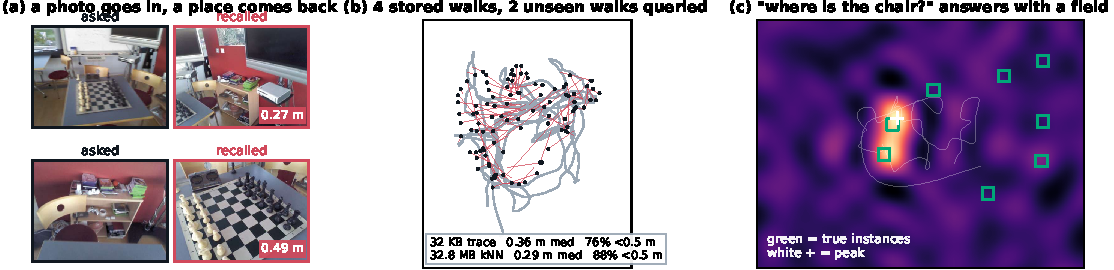
\includegraphics[width=\textwidth]{figures/reloc.pdf}
\caption{Cross-traverse relocalisation on 7-Scenes \texttt{chess}.
\textbf{(a)} Query frames from the two unseen test walks beside the
frames the 32\,KB trace recalled, at the 50th and 75th error percentile
so the panel shows typical rather than best behaviour.
\textbf{(b)} Every test query: the four stored training walks (grey),
each query's true position (dot), and a segment to the answered position
(red). The tail is left visible, and the box reports the median together
with the fraction within 0.5\,m for the trace and for exact nearest
neighbour over the same descriptors at 1000$\times$ the bytes.
\textbf{(c)} An object-class query on Replica \texttt{room0} decoded over
the floor plane: the peak (white cross) lands on a true instance.}
\label{fig:reloc}
\end{figure*}

\begin{table}[t]
% provenance: tracker (ax); outputs/cross_recall_7scenes_chess.json
\caption{7-Scenes \texttt{chess}, official cross-traverse split
(memory = 4 train traverses, queries = 2 test traverses; EigenPlaces
z-scored; $D$=8192). 3D error is the retrieved frame's translation
error. Trace bytes are phase-only (one float32 per dimension,
Sec.~\ref{sec:traces}); under the complex64 FHRR convention
\cite{snyder2026hyperspace} the trace reads 64\,KB and the comparison is
unchanged in kind.}
\label{tab:chess}
\centering
\small
\begin{tabular}{@{}lrrrr@{}}
\toprule
System & Bytes & 3D med. & \multicolumn{2}{c}{2D fraction} \\
 & & & $\le$0.5\,m & $\le$1\,m \\
\midrule
kNN exact (ceiling) & 32.8\,MB & 0.29\,m & 88.5\% & 98.1\% \\
PQ $m{=}8$ & 2.1\,MB & 0.29\,m & 89.6\% & 98.5\% \\
\textbf{VSA trace} & \textbf{32\,KB} & \textbf{0.36\,m} & 76.4\% & 93.0\% \\
VSA top-3 (2D) & 32\,KB & -- & 91.5\% & 98.9\% \\
\bottomrule
\end{tabular}
\end{table}

The conditioning mechanism replicates on this public benchmark: the raw
trace reaches only 0.75\,m median 3D versus 0.37/0.36\,m centred/z-scored.
Two scoped nuances, both measured: whitening is harmless \emph{here}
(0.34\,m) though strongly harmful elsewhere
(Sec.~\ref{sec:conditioning}), so the claim is scene/encoder-dependent
and we never state it universally; and binding heading mildly helps the
tail on this orbit-style scene (argmax $\le$1\,m: 93.0\%$\to$97.9\%)
because the trajectory makes heading informative, so the substitution
law's ``uninformative key'' clause is trajectory-dependent.

\emph{Multi-session merge, real sessions:} four session memories built
independently from the four training traverses and summed agree with the
jointly built trace to max $|\Delta| = 1.6\times10^{-15}$ and answer all
2{,}000 test queries identically.
% provenance: tracker (ax), merge check in cross_recall.py --merge-check

\subsection{Object grounding on eight Replica scenes: memory at the
perception ceiling}
\label{sec:grounding}

We characterise the object memory with a protocol of our own design and
label it as such (Sec.~\ref{sec:setup}, rule 4): store the YOLO+depth
object stream (bounded insertion, one 32\,KB trace per scene,
2{,}357--10{,}465 observations); query each ground-truth-comparable
class (Fig.~\ref{fig:fields}); an answer grounds correctly if the decoded
position lies within $r$ of a true instance of that class, with
Monte-Carlo chance anchors.
Pooled over 8 scenes and 42 scoreable GT classes (37 of 42 ground
correctly at $r$=1\,m): 88.1\% at $r$=1\,m (chance 18.2\%) and 78.6\%
at $r$=0.5\,m (chance 5.9\%).
% provenance: tracker (bd); outputs/replica_truth_aggregate.json
These are \emph{characterisation} numbers: the protocol is bespoke, so
they support internal comparisons only; the benchmark-native semantic
comparison is below.

Three internal comparisons carry the finding. \emph{(1) Miss taxonomy:}
of 5 pooled misses, 2 are classes the detector never saw and 3 are wrong
label/depth on the stored observation; \textbf{memory-attributable
misses are zero}. \emph{(2) Backend ablation at a fixed frontend:} on the
identical observation stream, the 32\,KB trace (89\% scene-mean) matches
or beats an explicit instance list (86\%) and a raw observation store
(81\%); on \texttt{office1} the trace grounded a table from a single
stored observation that the clustering backend's minimum-count rule
discarded. The trace gives nothing away to the structures it undercuts in
size, and the errors that remain belong to perception. \emph{(3)
Vocabulary coverage stated:} the COCO-80 detector sees only 9--31\% of GT
instances per scene; the battery examines that subset honestly, and an
independent CLIP labeler (agreement gate) removes consistent detector
hallucinations: on \texttt{room0} it deletes 1{,}212/5{,}359
observations and the phantom classes they created.

\emph{Benchmark-native comparison (adopted metric).} For the semantic
head-to-head we run ConceptGraphs' own evaluation (their scorer, their
ground truth, both systems producing the same output type). We evaluate
on all 8 scenes of the standard NICE-SLAM/vMAP Replica render release
--- the same data format their pipeline consumes --- but ConceptGraphs'
own paper reports Replica results on 7 of these (\texttt{room0-2},
\texttt{office0-3}, no \texttt{office4}): confirmed for their scene-graph
construction table and consistent with every other Replica experiment in
their paper, though their semantic-segmentation table does not restate
the scene count next to it. We therefore report the 7-scene subset as
the direct comparison against their published $\sim$0.40 mAcc
\cite{gu2024conceptgraphs}, with the full 8-scene number reported
alongside as broader coverage --- \texttt{office4} has no published
ConceptGraphs baseline to compare against. Pre-registered expectation,
stated before the run and confirmed: under their \emph{all-classes}
dense-labelling metric our object memory scores $\approx$0.076 mAcc on
\texttt{room0}, because wall/floor/ceiling dominate the points and a
detector-fed object memory cannot label them. All comparison rows below
therefore use their own object-class convention (\texttt{n\_exclude} 6,
verified against their evaluation code rather than their paper), and
the gap's sign is stable across all three of their published exclusion
settings (\texttt{n\_exclude} 1/4/6: $-$0.060/$-$0.070/$-$0.078 mAcc).

The run landed after two bugs in \emph{our} scoring of \emph{their}
system were found and fixed --- we had selected their map file by size
where their post-processing pass \emph{removes} points, and we had
omitted their in-scene class restriction; both bugs flattered us. With
their protocol reproduced faithfully, our measurement of their released
pipeline lands at 0.402 mAcc / 0.356 F-mIoU against their published
0.406 / 0.360 (98.9\% / 99.1\%, both metrics), which is what makes the
comparison quotable. Both systems then consume the identical SAM+CLIP
frontend stream; only the memory differs.

\begin{table}[t]
% provenance: outputs/batch1/table2_full.json (their scorer, 5 seed
% tuples; ours_seed_sd mean 0.017); 7-scene cut = no office4
\caption{Replica head-to-head under ConceptGraphs' own evaluation.
Ours is one fixed 32\,KB trace per scene; theirs an unbounded
point-cloud map. Mean over scenes; our across-seed sd averages 0.017.}
\label{tab:replica}
\centering
\small
\begin{tabular}{@{}lcccc@{}}
\toprule
 & \multicolumn{2}{c}{7-scene matched} & \multicolumn{2}{c}{8-scene full} \\
 & mAcc & F-mIoU & mAcc & F-mIoU \\
\midrule
published \cite{gu2024conceptgraphs} & -- & -- & 0.406 & 0.360 \\
ConceptGraphs, measured & 0.370 & 0.376 & 0.402 & 0.356 \\
\textbf{32\,KB trace (ours)} & 0.303 & 0.299 & 0.324 & 0.280 \\
\bottomrule
\end{tabular}
\end{table}

The bounded memory holds 0.80$\times$ their mAcc, leads outright on two
of eight scenes (\texttt{room2}, \texttt{office1}; paired sign test
$p$=0.29, direction consistent), and the deficit is \emph{located}
rather than diffuse. Per-cell forensics over every cell we lose
attribute 62\% to observation-stream label placement --- cells where the
stream's own nearest label is the wrong class, which no memory backend
can repair (any local decoder over the same stream answers the same
wrong class there) --- and 38\% to competitions inside one kernel
length-scale: the GT class's nearest observation sits at a median
4\,cm from the cell and the winner's at 15\,cm, both inside
$\ell$=0.45\,m, where a continuous point cloud resolves the
centimetre-scale interleaving and a kernel readout cannot
(\texttt{sofa}$\to$\texttt{cushion}, physically interleaved objects, is
29\% of this branch alone). Capacity is not the binding constraint:
mAcc moves $\sim$0.06 across a 32$\times$ trace-size range (4--128\,KB),
though F-mIoU still climbs over the same range, so both metrics are
quoted.

\emph{Degradation, the thesis measured.} The same degradation is
applied to the shared input stream at matched rates --- sparse coverage,
label corruption, pose jitter --- and each system re-runs its own
prediction rule. At the worst level the trace retains 76--94\% of its
own clean score where the point-cloud map retains 45--52\%, and the
crossover is \emph{absolute}, not merely relative: in all nine
scene$\times$mode sweeps tested (3 scenes $\times$ 3 modes) the 32\,KB
trace ends above the unbounded map's raw score, e.g.\ \texttt{office4}
at 5\% coverage 0.354 vs.\ 0.224, under 0.5\,m jitter 0.430 vs.\ 0.307.
Superposition averages a corrupted observation into near-orthogonal
noise that cleanup absorbs; an explicit nearest-neighbour structure has
no averaging, so each bad point is simply wrong wherever it is closest.
The same kernel smoothing that costs the 38\% sub-resolution deficit
above is what buys this robustness --- two faces of one
representational choice.
% provenance: outputs/batch1/table2_full.json, table2 sign test;
% outputs/degradation_sweep.json (9/9 absolute crossovers verified);
% outputs/batch1/local_loss_forensics.json (62/38 split, medians);
% wiki/analysis/2026-08-17-gap-closing-batch-results.md (corrected
% 2026-08-18 mechanism section)

Their query-style protocol (R@1/2/3 over text queries) remains the
adopted shape for a future object-retrieval comparison; its 20
affordance/negation query strings are published in their Appendix A4,
but the relevance judgements are not, so that comparison awaits our own
re-annotation and is reported separately when it exists.

\begin{figure}[t]
\centering
\todo{Figure: belief-field montage: 2--3 Replica class queries
(field heatmap over floorplan + GT squares + answer crosses), one
consistent-but-false case. Harvest from
\texttt{outputs/grounding\_inspector\_*.html} payloads.}
\caption{Spatial belief fields for class queries on Replica. The field is
the map state's full answer; argmax is one readout.}
\label{fig:fields}
\end{figure}

\subsection{Map merging: addition versus association}
\label{sec:merge-results}

Four simulated robots each observe a disjoint contiguous quarter of a
scene's trajectory; their maps must become one. Table~\ref{tab:merge}
compares merge operators over \emph{identical} observation streams,
truth-scored, averaged over the 8 scenes.
% provenance: tracker (bd),(bc); merge_comparison_k4.json per scene;
% survey: wiki/analysis/2026-08-05-map-joining-vs-alternatives.md
The instance-list row is the scene-graph merge in miniature: 622 greedy
association decisions across the sweep, with wrong ones costing up to 16
points on a scene; the merge step itself is where accuracy dies, which
is exactly the failure mode multi-robot scene-graph systems build
machinery to fight \cite{chang2023hydramulti}. VSA-OGM
\cite{snyder2026vsaogm} demonstrates the same additive merge for
occupancy and reports fused accuracy; the comparison here is the one it
does not run --- the same observations merged by association --- and the
column it does not report, agreement with the jointly built map. The
trace cannot make an
association error because there are no associations; four robots each
transmit one 32\,KB vector where a Kimera-Multi experiment moves
24--146\,MB \cite{tian2022kimeramulti}; the problems solved differ
(they also estimate the frame; see below), but it is the right scale
bar.

\begin{table}[t]
\caption{4-robot map joining on identical observations, mean over 8
Replica scenes (grounding R@1 at 1\,m, internal protocol).}
\label{tab:merge}
\centering
\small
\begin{tabular}{@{}lrrrr@{}}
\toprule
Join method & Bytes/robot & Assoc. & Mean (worst) & Exact? \\
\midrule
\textbf{VSA trace + addition} & 32\,KB & 0 & \textbf{89\% (80\%)} & $\sim$10$^{-12}$ \\
Instance lists + assoc. & 0.3\,KB & 622 & 84\% (67\%) & drifts \\
Count grids + addition & $\sim$95\,KB & 0 & 82\% & exact \\
Raw observation union & grows & 0 & 85\% & exact \\
\bottomrule
\end{tabular}
\end{table}

\emph{The standing caveat.} Exactness is conditional on a shared atom
vocabulary and a shared coordinate convention. The classical machinery we
bypass exists to \emph{recover} the unknown inter-robot transform; the
algebra assumes the frame, it does not solve it, and misaligned traces
sum to inconsistent superposition with no error signal. The fair reading
of Table~\ref{tab:merge} is against the back-end merge step of prior
systems, still iterative and inexact even given the frame, not
against their front-ends.

\subsection{The memory bounds odometric drift}
\label{sec:kalman-results}

Both steps of a Kalman-style filter are native to the algebra: predict is
one bind (Eq.~\eqref{eq:homo} moves the belief by the odometry increment,
$O(D)$, no grid), update is one bundle,
$S_{\text{post}} = \operatorname{norm}(a\,S_{\text{meas}} +
(1-a)\,S_{\text{pred}})$; decoding is needed only for display. Odometry
is corrupted with per-step noise plus systematic bias (propagating true
deltas would be trivially perfect). Classroom sequence, 10 noise draws:
% provenance: tracker (ag),(ah); vsa_kalman_seeds.json
filtered error \textbf{0.364$\pm$0.051\,m} versus dead
reckoning 0.868$\pm$0.503\,m at the lowest noise; physically impossible
jumps 242 $\to$ 6.5$\pm$2.4. Sweeping odometry quality 20$\times$
(Table~\ref{tab:kalman}), dead reckoning diverges to 17.6\,m while the
fused estimate saturates at 0.62\,m, approximately the memory's own
recall accuracy. That is the mechanism, stated plainly: the honest claim
is not that the memory out-localises odometry (raw recall, median
0.62\,m, does not reliably beat low-noise dead reckoning:
0.87$\pm$0.50\,m over 10 noise seeds, dead reckoning winning 5 of 10)
but that \emph{a fixed-size associative memory caps unbounded drift at
$O(D)$ per frame}. The optimal
gain rises monotonically with noise, as filter theory requires.

\begin{table}[t]
\caption{Drift bounding under odometry degradation (classroom, DINOv2
crops z-scored, blocked memory of 814 frames; medians over 10 noise
draws for the headline row, sweep rows single-draw with best gain).}
\label{tab:kalman}
\centering
\small
\begin{tabular}{@{}lrr@{}}
\toprule
Odometry noise $\sigma$ & Dead reckoning & Best filtered \\
\midrule
0.02 & 0.87\,m & \textbf{0.35\,m} \\
0.10 & 3.80\,m & \textbf{0.63\,m} \\
0.40 & 15.2--17.6\,m & \textbf{0.62--0.63\,m} \\
\bottomrule
\end{tabular}
\end{table}

\subsection{Conditioning ablations}
\label{sec:ablations}

The treatment ordering (centre or z-score $>$ raw $\gg$ whiten)
replicates across three scenes and three query types (position,
position-given-heading, time). Classroom EigenPlaces, blocked splits, 5
seeds, 744 queries:
% provenance: tracker (aw); heldout_eval_eigenplaces_5seed.json;
% time recall: tracker (ar),(au); outputs/school_run1/time_recall.json
raw 2.05$\pm$0.77\,m median, centred
0.87$\pm$0.24, z-scored \textbf{0.84$\pm$0.21} (79.8$\pm$6.5\% of the
chance--oracle gap), whitened-128 4.57$\pm$0.36 ($-47.6\%$, worse than
a constant predictor). Time recall on an 11{,}211-frame school traverse
reproduces the ordering at 10k scale (centred 43.5$\pm$12.3\% vs raw
23.5$\pm$8.1\%, whitened 1.1$\pm$13.2\%). The key-diversity substitute
and its scope conditions are in Sec.~\ref{sec:conditioning}. The
frontend swap itself (DINOv2 crops $\to$ EigenPlaces) is a solid 5-seed
improvement (1.14$\to$0.84\,m median), so descriptor choice and
conditioning contribute separately.

% =========================================================================
\section{Limitations}
\label{sec:limitations}

\textbf{Instance identity.} Binding class$\bnd$position recalls
\emph{class} fields: on multi-instance classes the argmax lands on the
wrong instance 72\% of the time (1{,}309 held-out instance queries over 5
scenes; internal diagnostic). Using each observation's own appearance
phasor as the key raises instance accuracy to 43\% and a hybrid cuts
outright errors to 3\%, but part of the residual is Replica's genuinely
identical instance models, which no appearance key can individuate.
Relational query interfaces over the trace (``the chair near the lamp'')
are under active study and remain internally-diagnosed only; systems with
explicit relational structure \cite{farm2026} currently hold this
frontier.

\textbf{Vocabulary and metric coverage.} The object memory sees what its
detector sees (9--31\% of Replica GT instances under COCO-80), and cannot
label structure classes; our pre-registered expectation under the
dense all-classes metric is accordingly low
(Sec.~\ref{sec:grounding}).

\textbf{The shared frame.} Merge exactness assumes a shared coordinate
convention (Sec.~\ref{sec:merge-results}); frame recovery inside the
algebra (correlation over the FPE group) is built but its robustness
under partial overlap is unmeasured, so no claim is made.

\textbf{Scale and scope.} Room-scale scenes, $\sim$10$^4$ observations per
trace, one self-collected platform for the filter experiments;
single-split headline numbers carry seed tags, and the 5-seed spread on
the classroom shows split-friendliness effects of $\sim$2$\times$.
Whitening's harm and heading's value are scene- and
trajectory-dependent and stated as scoped claims. Absolute recall is
honest-modest everywhere: the memory tracks its frontend's ceiling; it
does not exceed it.

% =========================================================================
\section{Conclusion}
\label{sec:conclusion}
% MERGE NOTE: complete draft; merge with the Overleaf partial.

We characterised a spatial-semantic map whose entire state is one
fixed-size vector: insertion is a multiply-add, a family of
object/place/time queries is one unbind each, and merging maps from
multiple sessions or robots is elementwise addition: exact, with zero
association decisions, measured against the association-based alternative
on identical observations. On a public relocalisation benchmark the trace
recalls within 0.07\,m of exact nearest neighbour at $\sim$1000$\times$
fewer bytes, in a size regime where standard compression cannot follow;
on eight Replica scenes its grounding misses are entirely attributable to
perception; against a reproduced ConceptGraphs baseline under that
system's own evaluation it holds 0.80$\times$ the accuracy of an
unbounded map on clean input and overtakes it outright in every
degraded-input condition tested; and its interference is governed by a
capacity law precise enough to predict a held-out condition to 1.4\%,
to diagnose a deployed failure, and to predict the direction of its
fix. The law also supplies the
deployment discipline (condition the content stream or bind a diverse
key; cap per-class insertion) that makes the algebra work on real
learned features.

The trade is stated as plainly as the wins: the representation is
bounded, associative, and approximate, where scene graphs are exact,
mutable, and relational. It does not solve the shared-frame problem its
merge operator assumes; it does not individuate identical instances; and
its recall ceiling is its perception's. What it offers robotics is a
map whose costs are known in advance: bytes fixed before deployment,
update cost independent of map age, merge cost independent of map
content, and failure modes predicted by an equation rather than
discovered in the field. Next steps are the benchmark-native semantic
head-to-head (pre-registered here), frame recovery inside the algebra,
and the relational query layer.

% =========================================================================
\section*{Acknowledgments}
% Standard Telluride acknowledgement, taken from the workshop site
% (sites.google.com/view/telluride-2026), which gives the sponsor list and
% grant numbers below; the site's "material in this website" is adapted to
% "material in this paper", which is the usual NSF boilerplate form.
This work was begun at the 2026 Telluride Neuromorphic AI Workshop, and
the authors thank its organisers and participants for the environment in
which the collaboration was formed. The material in this paper is based
upon work supported by the National Science Foundation under BCS 1824198,
OISE 2020624, and ECCS-2332166, and by ONR grant N00014-24-1-2025. Any
opinions, findings, and conclusions or recommendations expressed in this
publication are those of the authors and do not necessarily reflect the
views of the National Science Foundation.
\todo{institutional funding for each author; add any grant that supports
the Western Sydney, J{\"u}lich/RWTH, George Mason or CU Boulder
contributions}

\bibliographystyle{IEEEtran}
\bibliography{refs}

\end{document}
